% Copyright (C) 2005-2015 Airbus - EDF - IMACS - Phimeca
% Permission is granted to copy, distribute and/or modify this document
% under the terms of the GNU Free Documentation License, Version 1.2
% or any later version published by the Free Software Foundation;
% with no Invariant Sections, no Front-Cover Texts, and no Back-Cover
% Texts.  A copy of the license is included in the section entitled "GNU
% Free Documentation License".
\renewcommand{\filename}{docUC_InputNoData_DistManipulation.tex}
\renewcommand{\filetitle}{UC : Manipulation of a distribution}

% \HeaderNNIILevel
% \HeaderIILevel
\HeaderIIILevel


\label{manipulation_distribution}


\index{Copula!Estimation from sample}
\index{Mixture}
\index{Graph!Specifying the file format}
\index{Graph!PDF-CDF curves}
\index{Graph!PDF-CDF isocurves}
\index{Graph Manipulation!Bounding box}
\index{Graph Manipulation!View}
\index{Graph Manipulation!Show}
\index{Quantile!Distribution evaluation}
\index{Sample Statistics!Sample Generation}



The objective of this Use Case is to describe the main functionalities that OpenTURNS enables to manipulate a distribution of dimension $n \geq 1$.\\



Let's note $\vect{X} = (X_1, \cdots, X_n)$ the random vector associated to that distribution, which PDF is note $p$. OpenTURNS enables :
\begin{itemize}
\item to ask for the dimension, with the method {\itshape getDimension};
\item if $n >1$, to extract the extracted distribution of dimension $k<n$ corresponding to $k$ 1D marginals, with the method {\itshape getMarginal};
\item to get the copula, with the method {\itshape getCopula}: if the distribution is of type ComposedDistribution, the copula is the one specified at the creation of the ComposedDistribution. If the distribution is not that sort (for example, a KernelMixture, a Mixture, a RandomMixture), the copula is computed from the Sklar theorem;
\item to ask for some properties on the copula, with the method {\itshape hasIndependentCopula, hasEllipticalCopula}, only for the types Usual Distribution and ComposedDistribution (defined from the 1D marginals and a copula);
\item to evaluate the mean vector (potentially of dimension 1), the covariance matrix (potentially of dimension $1\times 1$), the standard deviation, skewness and kurtosis vectors (potentially of dimension 1), with the methods {\itshape getMean, getStandardDeviation, getCovariance, getKurtosis, getSkewness}, defined by the following expressions :
  \begin{align*}
    \left\{
      \begin{array}{lcl}
        \displaystyle \vect{E}[\vect{X}] & = & \displaystyle (E[X_1], \cdots, E[X_n]) \\
        \displaystyle \mat{StdDev}[\vect{X}] & = & \displaystyle (\sqrt{E[(X_1-E[X_1])^2]}, \cdots, \sqrt{E[(X_n-E[X_n])^2]}) \\
        \displaystyle \mat{Cov}[\vect{X}] & = & \displaystyle (E\left[(X_i-E[X_i])(X_j-E[X_j])\right])_{i,j} \\
        \displaystyle \vect{skewness}[\vect{X}] & = & \displaystyle (E\left[\left(\frac{(X_1-E[X_1])}{\sqrt{\Var{X_1}}}\right)^3\right], \cdots, E\left[\left(\frac{(X_n-E[X_n])}{\sqrt{\Var{X_n}}}\right)^3\right]) \\
        \displaystyle \vect{kurtosis}[\vect{X}] & = & \displaystyle (E\left[\left(\frac{(X_1-E[X_1])}{\sqrt{\Var{X_1}}}\right)^4\right], \cdots, E\left[\left(\frac{(X_n-E[X_n])}{\sqrt{\Var{X_n}}}\right)^4\right])
      \end{array}
    \right.
  \end{align*}
\item to evaluate the roughness, with the method {\itshape getRoughness}, defined by :
  \begin{align*}
    roughness(\vect{X}) = ||p||_{\cL^2} = \sqrt{\int_\vect{x} p^2(\vect{x})d\vect{x}}
  \end{align*}

\item to get one realization or simultaneously $n$ realizations, with the method {\itshape getRealization, getSample},
\item to evaluate the Cumulative Distribution Function (CDF), the complementary CDF, the Probability Density Function (PDF) on a scalar (1D distribution only), on a point or on a numerical sample with the method {\itshape computeCDF, computePDF},
\item to evaluate the probability content of a given interval, with the method {\itshape computeProbability},
\item to evaluate a quantile (or a group of quantiles) or a complementary quantile, (or a group of complementary quantile) with the method {\itshape computeQuantile}. If the distribution if of dimension $n>1$, the $p-$ quantile is the hyper surface in $\Rset^n$ defined by  $\{\vect{x}\in \Rset^n, F(x_1, \dots, x_n) = p \}$ where $F$ is the CDF. OpenTURNS makes the choice to return one particular point among these points : $(x_1^p, \dots, x_n^p)$ such that $\forall i, F_i(x_i^p) =  \tau$ where $F_i$ is the marginal of component $X_i$ and $F(x_1, \dots, x_n) = C(\tau, \dots, \tau)$ where $C$ is the distribution copula. Thus, OpenTURNS resolves the equation $ C(\tau, \dots, \tau)=p$ then computes $F_i^{-1}(\tau) = x_i^p$.\\
  Note that the point  $(x_1^p, \dots, x_n^p)$ belongs to the curve $(F_1^{-1}(s), \dots, F_n^{-1}(s))$. In dimension 2, OpenTURNS draws the curve $s \mapsto (F_1^{-1}(s), F_2^{-1}(s))$ and points the quantile of order $p$, with $p\in [p_{min}, p_{max}]$ discretized with $N$ points: see the method {\itshape drawQuantiles}.
\item to evaluate the derivative of the CDF or PDF with respect to the parameters of the distribution at a particular point, with the methods {\itshape computeCDFGradient, computePDFGradient},
\item to evaluate the characteristic function of the distribution, only for the following distributions : Chi2, Gamma, Laplace, Logistic, univariate Normal, Rayleigh, Triangular, univariate TruncatedNormal, Uniform, KernelMixture (which includes a KernelSmoothing without bound treatment), Mixture, RandomMixture;
\item to draw :
  \begin{itemize}
  \item for a 1D distribution : the PDF and CDF curves, with the methods {\itshape drawPDF, drawCDF},
  \item for a 2D distribution : the PDF and CDF iso-curves, with the methods {\itshape drawPDF, drawCDF}, and the PDF and CDF curves of its 1D marginals, with the methods {\itshape drawMarginal1DPDF, drawMarginal1DCDF} ,
  \item for a $nD$ with $n\geq 3$ distribution : the PDF and CDF of each 1D marginal, with the methods {\itshape drawMarginal1DPDF, drawMarginal1DCDF} and the PDF and CDF iso-curves for a specified 2D marginal, with the methods {\itshape drawMarginal2DPDF, drawMarginal2DCDF}.
  \end{itemize}
\end{itemize}

Let's note that it is possible to visualize a graph whithin the TUI without creating the associated files, thanks to the command {\itshape Show}.\\

\noindent%
\requirements{
  \begin{description}
  \item[$\bullet$] three distributions of dimension 1, 2 and 3 : {\itshape dist\_1, dist\_2, dist\_3}
  \item[type:] Distribution
  \end{description}
}
{
  \begin{description}
  \item[$\bullet$] graphes, numerical points, ...
  \end{description}
}

\textspace\\
Python script for this UseCase :

\inputscript{script_docUC_InputNoData_DistManipulation}

\textspace\\


We draw respectively  in Figures \ref{tulipe} and \ref{contour2D_example2} the iso-curves of the PDF of the two following  distributions :
\begin{itemize}
\item Distribution 1 : Mixture of Normal distributions of dimension 2
\item Distribution 2 : Composed Distribution, with a Gumbel copula and each marginal some mixture of normals of dimension 1.
\end{itemize}



\begin{figure}[H]
  \begin{center}
    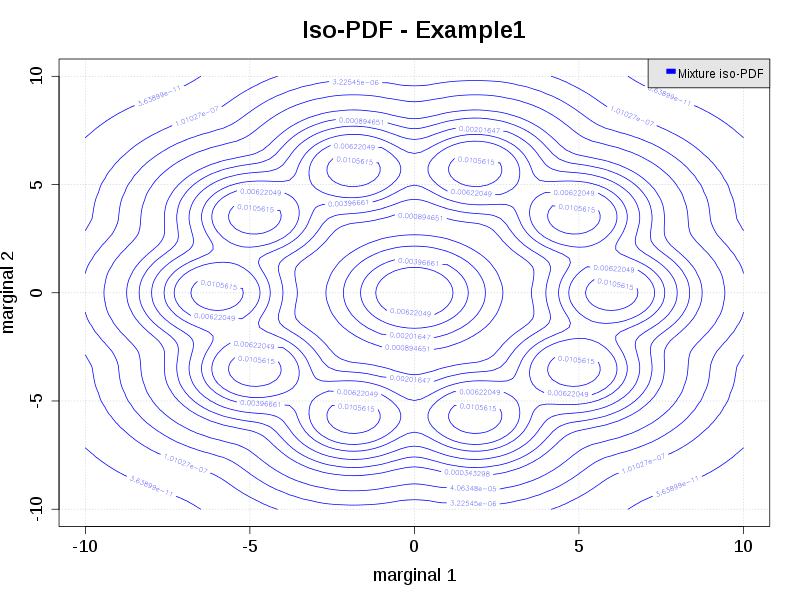
\includegraphics[width=10cm]{Figures/contour2D_tulipe.png}
  \end{center}
  \caption{Iso-curves of the PDF of Distribution 1 : Mixture of Normal distributions of dimension 2.}
  \label{tulipe}
\end{figure}

\begin{figure}[H]
  \begin{center}
    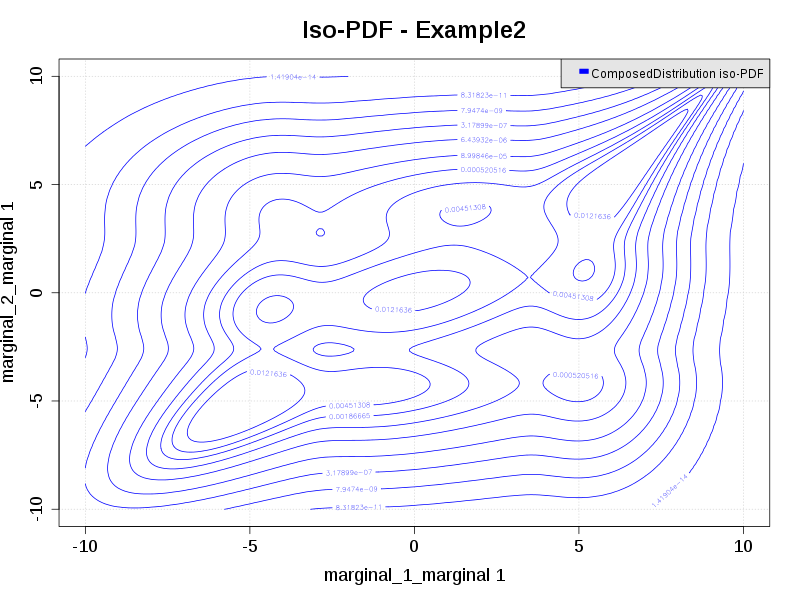
\includegraphics[width=10cm]{Figures/contour2D_2.png}
  \end{center}
  \caption{Iso-curves of the PDF of Distribution 2 : Composed Distribution, with a Gumbel copula and each marginal some mixture of normals of dimension 1.}
  \label{contour2D_example2}
\end{figure}

In the Figure \ref{quantileCurve}, we draw the quantile curve $p \mapsto F_1^{-1}(p)$ where  $p\in[0.1, 0.9]$ of the univariate $\cN(0,1)$ distribution.\\

In the Figure \ref{quantileCurve2d}, we draw the curve  $s \mapsto (F_1^{-1}(s), F_2^{-1}(s))$  and we point the quantiles of order $p \in [0.1, 0.9]$ regularly discretized into 101 points, of the bivariate distribution defined by: the margins are respectively  $\cN(0,1)$ and Triangular(0.0, 2.0, 3.0) and the copula is the Clayton copula($\theta=2.3$).


\begin{figure}[H]
  \begin{minipage}{9cm}
    \begin{center}
      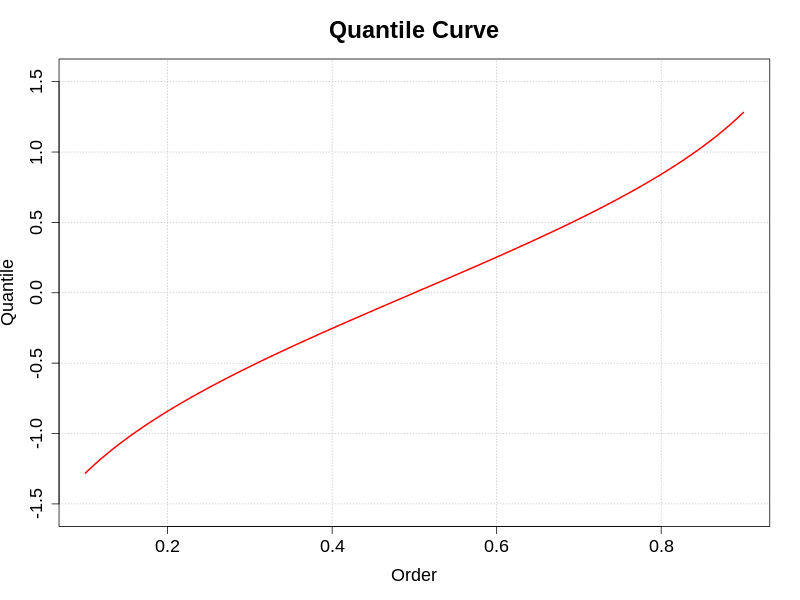
\includegraphics[width=7cm]{Figures/QuantileCurve2.png}
      \caption{A quantile curve in dimension 1.}
      \label{quantileCurve}
    \end{center}
  \end{minipage}
  \hfill
  \begin{minipage}{9cm}
    \begin{center}
      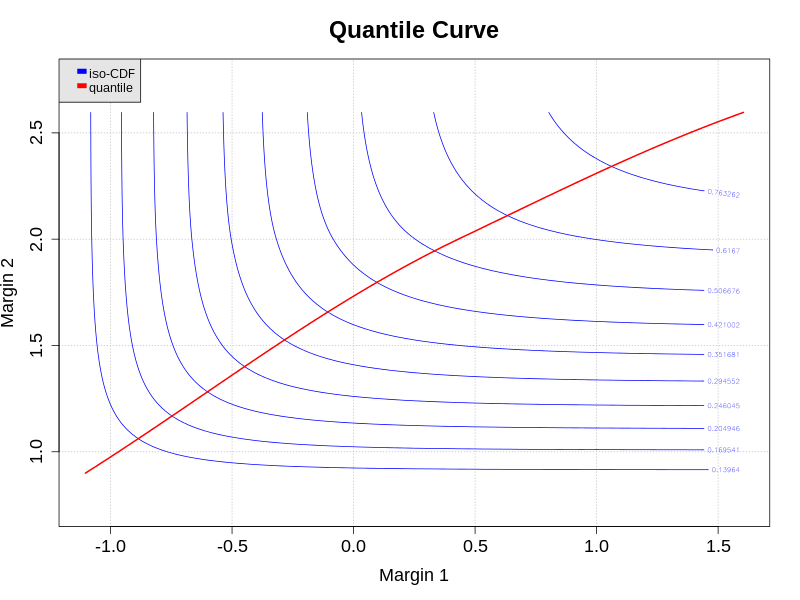
\includegraphics[width=7cm]{Figures/QuantileCurve.png}
      \caption{A quantile curve in dimension 2.}
      \label{quantileCurve2d}
    \end{center}
  \end{minipage}
\end{figure}
